\section{Variational Autoencoder (VAE): Học Không gian Tiềm ẩn}
\label{sec:vae}

\subsection{Giới thiệu: Cái thiếu sót của Autoencoder Thông thường}
\label{subsec:vae_intro}

Trước khi nói đến VAE, hãy nói về \textbf{Autoencoder (AE)} — tiền thân của nó.

Một Autoencoder là mạng nơ-ron được huấn luyện để nén dữ liệu vào một không gian chiều thấp hơn gọi là \textbf{không gian tiềm ẩn (latent space)}, rồi tái tạo lại dữ liệu gốc từ biểu diễn nén đó. Kiến trúc bao gồm:
\begin{itemize}
    \item \textbf{Encoder} $q_\phi(\mathbf{z}|\mathbf{x})$: Ánh xạ ảnh đầu vào $\mathbf{x}$ thành vector tiềm ẩn $\mathbf{z}$.
    \item \textbf{Decoder} $p_\theta(\mathbf{x}|\mathbf{z})$: Ánh xạ $\mathbf{z}$ trở lại ảnh tái tạo $\hat{\mathbf{x}}$.
\end{itemize}

Mạng được huấn luyện để cực tiểu hóa sai số tái tạo $\|\mathbf{x} - \hat{\mathbf{x}}\|^2$.

Autoencoder học được biểu diễn nén hữu ích, nhưng có một vấn đề nghiêm trọng nếu ta muốn dùng nó \textit{sinh ảnh mới}: không gian tiềm ẩn $\mathbf{z}$ không có cấu trúc. Các điểm trong $\mathbf{z}$-space bị phân bố tùy tiện — lấy một điểm ngẫu nhiên từ $\mathbf{z}$-space và decode nó ra, ta thường nhận được ảnh vô nghĩa.

\begin{center}
    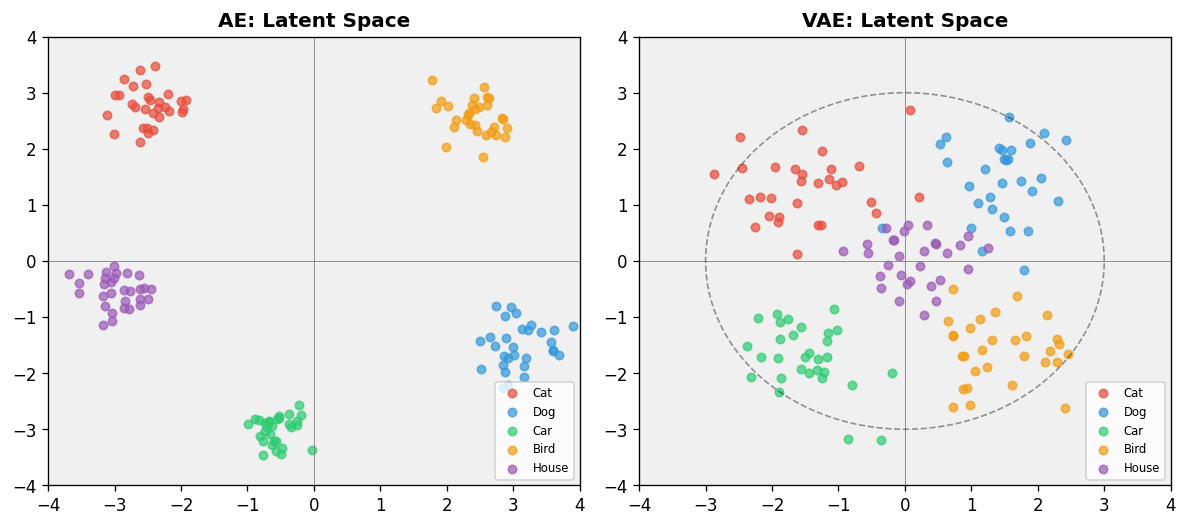
\includegraphics[width=0.85\textwidth]{images/ae_vs_vae_latent_space.png}
    \captionof{figure}{So sánh không gian tiềm ẩn của AE và VAE. (Trái) AE: các cụm dữ liệu phân bố rời rạc, không có cấu trúc — lấy mẫu ngẫu nhiên từ vùng trống sẽ cho kết quả vô nghĩa. (Phải) VAE: các cụm phân bố dày đặc và liên tục, việc lấy mẫu và nội suy cho kết quả có ý nghĩa.}
    \label{fig:ae_vs_vae_latent}
\end{center}

\subsection{Ý tưởng Xác suất: Học Phân phối thay vì Điểm}
\label{subsec:vae_idea}

\textbf{Variational Autoencoder (VAE)} \cite{Kingma2014} của Kingma và Welling giải quyết vấn đề này bằng một thay đổi tư duy mang tính cách mạng:

\begin{quote}
    \textit{Thay vì ánh xạ một ảnh $\mathbf{x}$ thành một \textbf{điểm} duy nhất $\mathbf{z}$ trong latent space, hãy ánh xạ nó thành một \textbf{phân phối xác suất} $q_\phi(\mathbf{z}|\mathbf{x})$.}
\end{quote}

Cụ thể, encoder của VAE xuất ra hai vector: \textbf{trung bình} $\boldsymbol{\mu}$ và \textbf{log-phương sai} $\log \boldsymbol{\sigma}^2$, định nghĩa một phân phối Gaussian cho $\mathbf{z}$:
\[
    q_\phi(\mathbf{z}|\mathbf{x}) = \mathcal{N}(\mathbf{z};\, \boldsymbol{\mu},\, \boldsymbol{\sigma}^2 \mathbf{I})
\]

Trong quá trình huấn luyện, $\mathbf{z}$ được \textit{lấy mẫu} từ phân phối này trước khi đưa vào decoder.

\begin{mdframed}[style=infobox]
    \textbf{Trực giác cốt lõi}

    Bằng cách ánh xạ thành phân phối, VAE buộc latent space phải \textit{mượt mà và liên tục}: mỗi điểm trong latent space sẽ tương ứng với ảnh có ý nghĩa, và các điểm gần nhau trong latent space sẽ cho ra các ảnh tương tự nhau. Đây là tính chất lý tưởng để \textit{sinh ảnh}: chỉ cần lấy mẫu ngẫu nhiên từ $\mathcal{N}(0, \mathbf{I})$, decode ra, và thu được ảnh hoàn chỉnh.
\end{mdframed}

\subsection{Hàm Mất mát ELBO và Trick Tham số hóa lại}
\label{subsec:vae_elbo}

\subsubsection{Evidence Lower Bound (ELBO)}
\label{subsubsec:elbo}

VAE được huấn luyện bằng cách tối đa hóa \textbf{Evidence Lower Bound (ELBO)} — một cận dưới của log-likelihood của dữ liệu:

\begin{equation}
    \mathcal{L}_{\text{VAE}} = \underbrace{\mathbb{E}_{q_\phi(\mathbf{z}|\mathbf{x})}\left[\log p_\theta(\mathbf{x}|\mathbf{z})\right]}_{\text{Reconstruction Loss}} - \underbrace{D_{\text{KL}}\left(q_\phi(\mathbf{z}|\mathbf{x}) \| p(\mathbf{z})\right)}_{\text{KL Divergence}}
    \label{eq:vae_elbo}
\end{equation}

\begin{itemize}
    \item \textbf{Reconstruction Loss:} Đo lường mức độ decoder tái tạo lại $\mathbf{x}$ từ $\mathbf{z}$. Thường là Mean Squared Error (cho dữ liệu liên tục) hoặc Binary Cross-Entropy (cho ảnh nhị phân). Số hạng này thúc đẩy \textit{tái tạo chính xác}.

    \item \textbf{KL Divergence:} Đo lường sự khác biệt giữa phân phối hậu nghiệm (posterior) $q_\phi(\mathbf{z}|\mathbf{x})$ và phân phối tiên nghiệm (prior) $p(\mathbf{z}) = \mathcal{N}(0, \mathbf{I})$. Số hạng này thúc đẩy latent space \textit{có cấu trúc và liên tục} gần với một Gaussian chuẩn.
\end{itemize}

Với phân phối Gaussian, KL divergence có dạng tường minh:
\[
    D_{\text{KL}}\left(\mathcal{N}(\boldsymbol{\mu}, \boldsymbol{\sigma}^2) \| \mathcal{N}(0, \mathbf{I})\right) = -\frac{1}{2} \sum_{j=1}^{d}\left(1 + \log \sigma_j^2 - \mu_j^2 - \sigma_j^2\right)
\]

\subsubsection{Reparameterization Trick}
\label{subsubsec:reparameterization}

Có một vấn đề kỹ thuật: bước \textit{lấy mẫu} $\mathbf{z} \sim \mathcal{N}(\boldsymbol{\mu}, \boldsymbol{\sigma}^2 \mathbf{I})$ là phép toán ngẫu nhiên, không thể lan truyền ngược gradient qua đó.

Giải pháp là \textbf{Reparameterization Trick}: tách sự ngẫu nhiên ra khỏi luồng gradient bằng cách viết lại phép lấy mẫu như sau:
\[
    \mathbf{z} = \boldsymbol{\mu} + \boldsymbol{\sigma} \odot \boldsymbol{\epsilon}, \quad \boldsymbol{\epsilon} \sim \mathcal{N}(0, \mathbf{I})
\]
Bây giờ sự ngẫu nhiên nằm hoàn toàn trong $\boldsymbol{\epsilon}$ — một biến \textit{độc lập với tham số của mô hình}. Gradient có thể chảy qua $\boldsymbol{\mu}$ và $\boldsymbol{\sigma}$ một cách bình thường.

\begin{center}
    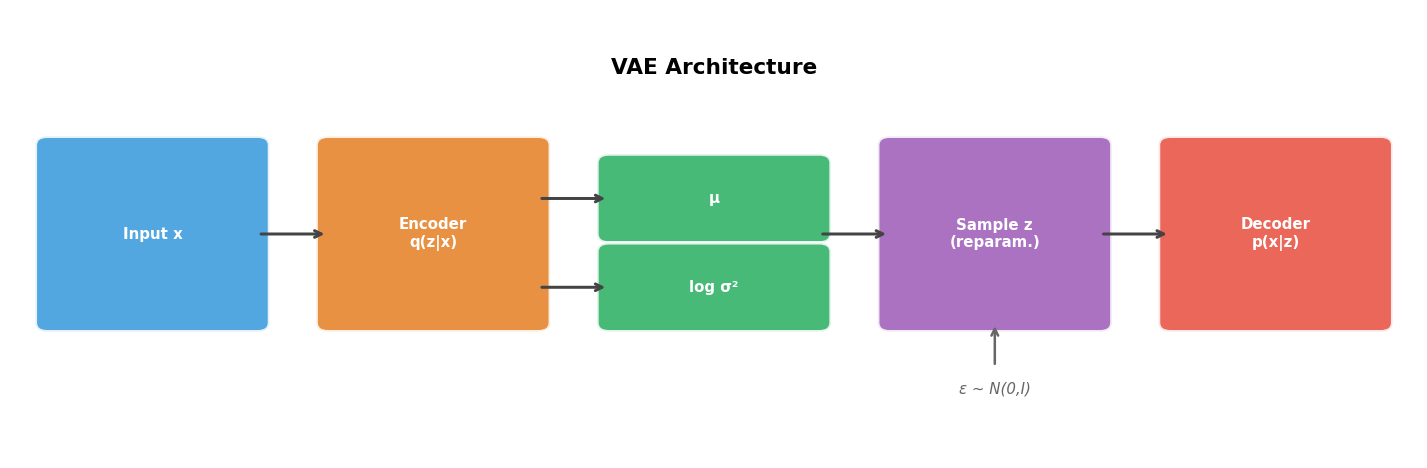
\includegraphics[width=0.9\textwidth]{images/vae_architecture.png}
    \captionof{figure}{Kiến trúc VAE. Encoder xuất ra $\boldsymbol{\mu}$ và $\boldsymbol{\sigma}$. Reparameterization trick lấy mẫu $\mathbf{z} = \boldsymbol{\mu} + \boldsymbol{\sigma} \odot \boldsymbol{\epsilon}$ (cho phép backprop). Decoder tái tạo ảnh từ $\mathbf{z}$. Hàm mất mát là tổng của reconstruction loss và KL divergence.}
    \label{fig:vae_architecture}
\end{center}

\subsection{VQ-VAE: Bước Tiến đến Mô hình Sinh Hiện đại}
\label{subsec:vqvae}

\textbf{VQ-VAE (Vector Quantized VAE)} \cite{VanDenOord2017} là một biến thể quan trọng: thay vì latent space liên tục, nó sử dụng latent space \textit{rời rạc} thông qua một codebook gồm $K$ vector:

\begin{enumerate}
    \item Encoder tạo ra biểu diễn liên tục $\mathbf{z}_e$.
    \item Mỗi vector trong $\mathbf{z}_e$ được "lượng tử hóa" thành vector gần nhất trong codebook: $\mathbf{z}_q = \arg\min_{e_k} \|\mathbf{z}_e - e_k\|$.
    \item Decoder nhận $\mathbf{z}_q$ và tái tạo ảnh.
\end{enumerate}

\begin{mdframed}[style=infobox]
    \textbf{Tại sao VQ-VAE quan trọng?}

    VQ-VAE chính là thành phần "nén ảnh" (image tokenizer) trong các mô hình sinh ảnh hiện đại nhất:
    \begin{itemize}
        \item \textbf{DALL-E} (OpenAI) dùng VQ-VAE để encode ảnh thành chuỗi token, sau đó dùng Transformer để tạo token mới.
        \item \textbf{Stable Diffusion} sử dụng một VAE để encode ảnh vào latent space nhỏ hơn, rồi chạy diffusion process trong latent space đó — tiết kiệm tính toán đáng kể so với diffusion trực tiếp trên pixel.
        \item \textbf{LLaVA, GPT-4V} dùng CLIP encoder (bản chất là encoder của CLIP, cũng học từ contrastive objective) để tokenize ảnh cho Language Model.
    \end{itemize}
    Hiểu VAE là hiểu kiến trúc nền tảng của toàn bộ hệ sinh thái generative AI hiện đại.
\end{mdframed}

\section*{Tài liệu tham khảo}
\begin{itemize}
    \item[1] Kingma, D. P.; Welling, M. Auto-Encoding Variational Bayes. In \textit{ICLR}, 2014.
    \item[2] Van Den Oord, A.; Vinyals, O.; Kavukcuoglu, K. Neural Discrete Representation Learning (VQ-VAE). In \textit{NeurIPS}, 2017.
    \item[3] Rombach, R. et al. High-Resolution Image Synthesis with Latent Diffusion Models. In \textit{CVPR}, 2022.
\end{itemize}
